\chapter{3D hand pose estimation}
\label{chap/hand}

\section{Introduction}

% Done  
Articulated 3D hand pose estimation is another important area in human activity analysis. 
It serves very different applications compared with body pose estimation, such as gesture and sign language recognition, user interface and computer graphics.
Nevertheless, articulated hand pose estimation shares a lot of similarities with 3D body pose estimation. Basically, both tasks aim to recognise the configuration of an articulated subject with high degrees of freedom. On the other hand, they require domain knowledge, \eg kinematics \cite{LaGorce2011, Simo-Serra2012}, specialised part detector \cite{Bissacco2007} or actions \cite{Yao2012}, in order to infer complex articulations from limited input data. 

% done 
While the latest depth sensor technologies have enabled body pose estimation in real-time \cite{Baak2011, Shotton2011, Girshick2011, Sun2012}, 3D hand pose estimation still remains an unsolved issue. Despite their similarities, proven approaches for body pose estimation cannot be repurposed directly to hand articulations, due to several unique characteristics of 3D hand pose estimation.  

% hand shapes 
\begin{figure}[th]
\centering
\begin{subfigure}[b]{0.22\linewidth}
	\centering
	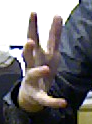
\includegraphics[height=4cm]{fig/hand/fig1_rgb.png}
	\subcaption{RGB image}
	\label{fig/hand/intro1}
\end{subfigure}
\begin{subfigure}[b]{0.22\linewidth}
	\centering
	
\includegraphics[height=3.5cm]{fig/hand/fig1_a.png}
	\subcaption{Joint labels}
	\label{fig/hand/intro2}
\end{subfigure}
\begin{subfigure}[b]{0.22\linewidth}
	\centering
	
\includegraphics[height=3.5cm]{fig/hand/fig1_c.png}
	\subcaption{Synthetic depth}
	\label{fig/hand/intro3}
\end{subfigure}
\begin{subfigure}[b]{0.22\linewidth}
	\centering
	
\includegraphics[height=3.5cm]{fig/hand/fig1_b.png} 
	\subcaption{Realistic depth}
	\label{fig/hand/intro4}
\end{subfigure}
\caption{\textbf{Example hand pose images.} From left to right, original RGB image, colour-coded joint labels, synthetically generated depth image, realistic depth image captured from a depth sensor.}
\label{fig/hand/intro}
\end{figure}

% done 
\begin{itemize} 

% done 
\item{\textbf{Occlusions and viewpoint changes}} \\  
Self occlusions are prevalent in hand articulations. The complex anatomy of the human hand provides at least 26 degrees of freedom \cite{Rehg1995, Holden1995}. Compared with limbs in body pose, fingers can perform more sophisticated articulations, leading to numerous possible observations. In addition, different from body pose that are usually upright and frontal \cite{Eichner2012}, varying camera viewpoints can render completely different depth images from the same hand articulation. 

% done 
\item{\textbf{Noisy input data}} \\ 
Body poses usually occupy larger and relatively static regions in the depth images. 
Hands, however, are often captured in a lower resolution, leading to more noisy inputs than body poses. 
Missing parts and quantisation errors are common in hand pose data, especially at small, partially occluded parts such as finger tips. Figure \ref{fig/hand/intro4} shows a depth image captured from a realistic environment, its hand shape is different from the synthetic depth image in figure \ref{fig/hand/intro3}.   
Regardless of the object distance, missing values are created when stereo image pairs fail to match on the occlusion boundaries, as shown in figure \ref{fig/hand/intro4}. 
Unlike sensor noise and depth errors \cite{Girshick2011, Baak2011}, these artefacts cannot be repaired or recovered easily. Consequently, a large discrepancy is observed between synthetic and realistic data.  

% done 
\item{\textbf{Inefficient data labelling}} \\ 
Due to noise, occlusions and the inherent complex structure of human hand, realistic data is extremely costly to obtain via manual labelling. 
Existing state-of-the-art methods leverage either synthetic data \cite{Keskin2012} or model-based visual tracking \cite{LaGorce2011, Oikonomidis2012}, to estimate hand poses without labelled training data. 
They do not consider the realistic-synthetic discrepancies. 
Despite achieving encouraging performances on synthetic testing data, these techniques give sub-optimal results when they are tested with realistic data. 
Furthermore, noisy realistic data makes automatic joint detection difficult, whereas in synthetic data, joint boundaries are always clean and accurate.
% Whilst handling shape variation is crucial for body pose estimation \cite{Shotton2011}, shape variations of human hands are generally smaller than that of body shape.        
\end{itemize} 

% done 
As a result, this work introduces the new \emph{Semi-supervised Transductive Regression} (\STR) forest to estimate 3D hand poses, by learning the relationship between realistic and synthetic data. 
The process of linking realistic and synthetic training data is known as \emph{transductive transfer learning} \cite{Pan2010}.  
A transductive model learns from a source domain, \eg synthetic data, during its training process.
It subsequently applies knowledge transfer to a different but related target domain, \eg realistic data, in the testing stage. 

% done  
The \STR\ forest learning algorithm is also semi-supervised. 
It learns the noisy appearances of realistic data from both labelled and unlabelled data points. 
As a result, it benefits from the characteristics of both domains. 
The \STR\ forest not only captures a wide range of poses from synthetic data, it also achieves robust performances in challenging environments by learning the noisy, irregular appearances of realistic data. 

% done 
In addition to the proposed \STR\ forest, a pseudo-kinematic joint refinement algorithm is proposed to handle occlusions and noisy articulations efficiently. 
Hypotheses of 3D hand pose estimates from the \STR\ forest are verified by this data-driven technique, which models the structure of human hands, without computing sophisticated inverse kinematics. 

% Why depth image not RGB 
% done 
Different from the action classification and body pose estimation in chapter \ref{chap/act} and \ref{chap/body}, the proposed system takes sequences of depth images as input rather than videos. 
Since the fingers and palm of a human hand share very similar texture, automatic segmentation of the hand is very difficult in traditional videos. 
In addition, due to occlusions and viewpoint changes, deformable part-based models used in chapter \ref{chap/body}, which require a stable holistic structure, becomes infeasible for hand pose estimation.   
Traditional video-based approaches rely on low-level silhouettes and edge features \cite{Rosales2001, Chua2002, Athitsos2003, Stenger2006}, which require extra computational effort in hand detection and segmentation and limited amount of recognisable poses.   
Depth images, on the other hand, provide straightforward hand and finger segmentation by providing 2.5D information of the scene. 
Although range sensors or stereo cameras are required to capture depth images, they are currently leveraged to optimise the performance of hand pose estimation. 

% done 
\subsection{Contributions} 
The main contributions of the proposed 3D hand pose estimation framework are as follows. 

% done, make this longer 
\begin{itemize}
\item{\textbf{Realistic-Synthetic fusion}}\\
Handling the issue of noisy inputs, a transductive learning algorithm for 3D hand pose estimation, namely the \STR\ forest, is proposed. The \STR\ forest relates the characteristics of realistic and synthetic training data, improving robustness and pose coverage in realistic testing environments.
\item{\textbf{Semi-supervised learning}}\\
Training a discriminative hand pose recogniser requires a large and extensive training dataset. Hand-labelling of hand pose data, however, is costly and ineffective due to occlusions and complicated articulations of human hands. 
The \STR\ forest utilises both labelled and unlabelled data in its learning algorithm, improving estimation accuracy while maintaining a low labelling cost. 
\item{\textbf{Data-driven pseudo-kinematics}}\\
	Traditional Hough forest algorithms do not model occlusions and structural consistency of articulations \cite{Gall2009}. A data-driven, pseudo-kinematic technique is therefore introduced to verify the feasibility of hand poses inferred from the preceding \STR\ forest.  
\end{itemize} 

\section{Related work}

% done 
\subsection{Hand pose estimation}

% done 
Approaches to 3D hand pose estimation are broadly categorised into generative and discriminative methods. In generative methods, a 3D articulated hand model is employed to evaluate the observed input for pose recovery. An appearance projection is synthesised from a hand pose hypothesis, which is registered to the current observation using a visual tracking or energy-minimisation algorithm. Various features, such as edges \cite{Guan2006}, silhouettes \cite{Wu2000}, optical flow \cite{Lu2003} and shading \cite{LaGorce2011} are used to guide the object registration process. Generative methods require no training and recognise a wide range of poses, yet the registration algorithms are usually computationally demanding and prone to tracking error.

% done 
Discriminative methods learn a mapping from visual features to 3D hand pose articulations through classification or regression techniques. A discriminative hand pose estimator is constructed from a training dataset offline, which is usually based on holistic shape features \cite{Rosales2001, Athitsos2003, Romero2009, Wang2009, Keskin2012}. Discriminative approaches are usually more efficient than generative approaches as no tracking is performed. Additionally, many discriminative methods are frame-based, such that they can recognise hand poses from a single image. However, discriminative approaches are restricted to a limited set of predefined poses, as they require a large labelled dataset for training, which is often very costly to obtain.  

% done 
\subsubsection{Early approaches} 
Earlier approaches to 3D hand pose estimation are diverse, different techniques have been applied to single images or videos. Erol \etal \cite{Erol2007} performed a detailed literature survey of hand pose estimation techniques. Chua \etal \cite{Chua2002} recognised hand poses from coloured markers on the hand to analyse hand articulations. Athitsos \etal \cite{Athitsos2003} estimated articulated hand and viewpoint from a database using probabilistic line matching. Tackling the problem of view ambiguities in hand poses, Guan \etal \cite{Guan2006} designed a multiple camera approach to infer 3D hand poses from contours. Stenger \etal \cite{Stenger2006} presented a model-based hand poses tracking algorithm using a Bayesian filter based on Chamfer matching.  

\subsubsection{Generative approaches} 
Generative approaches are more popular than discriminative approaches among recent state-of-the-art approaches, thanks to its ability to handle a wide range of articulations and viewpoint changes.   
In a generative hand pose estimation algorithm, hypotheses are projected from an articulated model, hand poses are tracked by fitting the hypotheses to the test data. 
For example, De La Gorce \etal \cite{LaGorce2011} used a hand mesh with detailed simulated texture and lighting. 
Hamer \etal \cite{Hamer2009} addressed strong occlusions using local trackers at separate hand segments. 
Ballan \etal \cite{Ballan2012} inferred finger articulations by detecting salient points.  
Oikonomidis \etal \cite{Oikonomidis2011} estimated hand poses in real-time from RGB-D images using particle swarm optimisation. 

Although no training data is required for the above generative approaches, visual tracking and optimisation have imposed several limitations to hand pose estimation.
Tracking performances depends on the previous pose estimations, output pose estimates may drift away from ground truth when errors accumulate over time. 
When tracking is eventually lost, accumulated incorrect pose estimates cannot be recovered without manual re-initialisation or re-detection. 
In addition, most generative methods do not consider shape variations among individuals due to the additional complexity involved, affecting their accuracy in realistic applications \cite{Erol2007}.   
Furthermore, their iterative optimisation processes are usually computationally expensive. Despite near real-time performance with the latest GPU acceleration techniques \cite{Oikonomidis2011}, generative methods struggle to attain real-time performance on commodity hardware. 

% Done 
\subsubsection{Discriminative approaches} 
Discriminative approaches learn a function that maps from visual features to pose, where the mapping is usually regarded as a classification or regression problem. As opposed to generative approaches that use a predefined visual model, discriminative models are constructed from a training dataset.   
In discriminative approaches, hand poses are often represented as holistic templates \cite{Wang2009}, joint labels \cite{Shotton2011} or joint coordinates \cite{Girshick2011}.
Although discriminative methods have proved successful in real-time body pose estimation from depth sensors \cite{Shotton2011, Girshick2011, Baak2011, Sun2012}, they are less common than generative approaches with respect to hand pose estimation.  
Recent discriminative algorithms for hand pose estimation include approximate nearest neighbour search \cite{Romero2009, Wang2009} and hierarchical random forests \cite{Keskin2012}.  

Run-time performance is the major advantage of discriminative approaches over generative approaches. They involve no iterative optimisation or visual tracking in their testing process, thus inference is usually more efficient than generative pose estimators.  
Discriminative models also handle shape variations more efficiently by generating extra synthetic training data with different shapes. Recently, the bottleneck of the feature extraction process is resolved using specialised hardware, \eg Kinect sensor \cite{Shotton2011}, achieving real-time performance for practical applications. Last but not least, many discriminative approaches are frame-based such that the drifting issue in generative approaches does not exist. 

Discriminative methods, however, rely heavily on training data. The number of recognisable poses of a model is correlated to the size of training dataset. In other words, the overall performance of a discriminative pose estimator is largely determined by its training dataset. 
Since it is costly to label sufficient realistic data for training, existing approaches resort to synthetic data by means of computer graphics \cite{Romero2009, Keskin2012}, leading to the problem of realistic-synthetic discrepancies.

% done 
\subsection{Inverse kinematics}   
Inverse kinematics has become a popular technique in optimisation-based and tracking-based  approaches for both body and hand poses estimation. 
Girshick \etal \cite{Girshick2011} estimated body poses using a simple range heuristic, but it is inapplicable to hand pose due to self-occlusions. 
Zhu \etal \cite{Zhu2008a} applied visual tracking and inverse kinematics to estimate simplified body poses from sequences of depth images.
Pons-Moll \etal \cite{Pons-Moll2011} presented a multi-camera motion capture system using Mises-Fisher sampling and inverse kinematics.  

However, applying inverse kinematics to hand pose estimation is not as straightforward as that of body pose. As previously mentioned, fingertips are occluded frequently due to self-occlusions, extracting their locations for inverse kinematics is difficult, especially in videos. 
Lacking a deformable articulated model, few discriminative methods consider the physical characteristics of human hands. For example, Wu and Huang \cite{Wu1999} searched for the optimal solution in inverse kinematics through a genetic algorithm. Additionally, Wang \etal \cite{Wang2009} proposed a data-driven approach to describe inverse kinematics using a colour-coded glove. The colour-coded glove avoided the problem of finger segmentation in video-based systems, a binary coding scheme was designed to perform a nearest neighbour search efficiently in a large synthetic database. 

Coping with the issues of occlusion and computational complexity, this work proposes a data-driven, pseudo-kinematic method to correct strongly occluded poses. Distributions of joint locations are efficiently described in a large database of synthetic hand articulations. Occluded joint centres are recovered by matching the visible joints from the corresponding distributions.

% done 
\subsection{Transfer learning} 
Transductive transfer learning is often employed when training data of the target domain is too costly to obtain. 
It has seen various successful applications \cite{Pan2010}, nonetheless it has not been applied to articulated pose estimation. 
In this work, realistic-synthetic fusion is realised by extending the idea of cross-modality learning by Bronstein \etal \cite{Bronstein2010} to the proposed \STR\ forest, where the training algorithm preserves the predefined associations between cross-domain data pairs, which are defined in section \ref{sec/hand/dataset}.  

% done 
\subsection{Semi-supervised forest and regression forest} 
Various semi-supervised forest learning algorithms have been proposed. Shotton \etal \cite{Shotton2013} measured data compactness to relate labelled and unlabelled data points. Leistner \etal \cite{Leistner2009} designed a margin metric to evaluate unlabelled data. On the contrary, a regression random forest was adopted in body pose estimation \cite{Girshick2011, Sun2012}. In the proposed system, a \STR\ forest adaptively combines the aforementioned semi-supervised and regression forest learning techniques in a single frame work.

\section{Overview}

% different shape --- apperance based 
\begin{figure}[ht]
	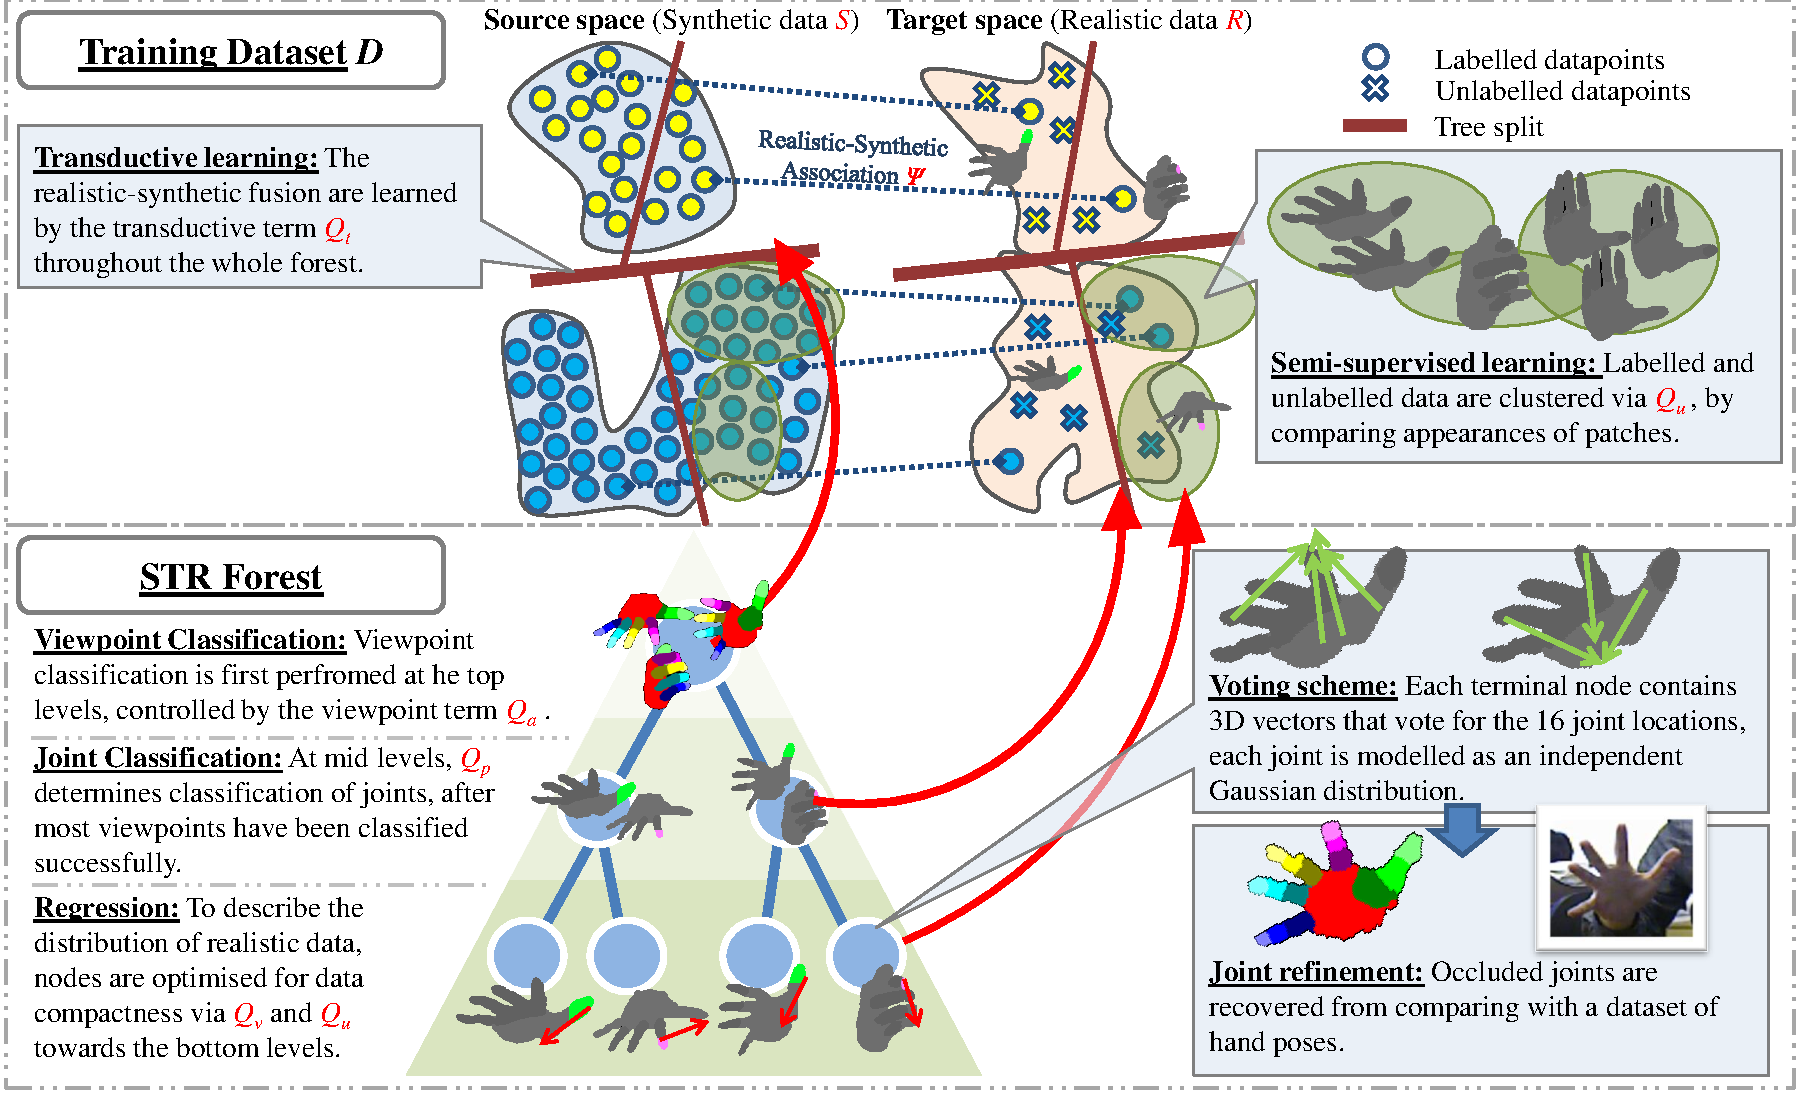
\includegraphics[width=1.00\linewidth]{fig/hand/overview.pdf}
	\caption{\textbf{The proposed \STR\ learning model.}}
	\label{fig/hand/concept}
\end{figure}

% done 
The concept of \STR\ learning is illustrated in figure \ref{fig/hand/concept}(top). 
Training data is collected from a target domain (realistic depth images) and a source domain (synthetic depth images). Whilst data points in the fully labelled source domains are generated automatically with ground truh, only a small portion of the data points in the target domain are labelled manually and the remaining points are left unlabelled. 
The synthetic dataset and the realistic dataset are related by establishing associations from the labelled target data points to their corresponding source data points, as shown in figure \ref{fig/hand/concept}. The proposed \STR\ learning algorithm introduces two new techniques to the traditional Hough and regression forest \cite{Gall2011}. 
Transductive realistic-synthetic associations is preserved throughout the learning process, such that the paired data points pass down to the same node. 
Furthermore, the distribution of labelled and unlabelled realistic data are described jointly in the proposed \STR\ forest using an unsupervised learning term. 

Extending the action detection forest in chapter \ref{chap/body}, the \STR\ forest is a hybrid random forest that performs classification and regression tasks adaptively within a unified algorithm. Figure \ref{fig/hand/concept}(bottom) shows the different tasks performed by \STR\ forest. At the top levels of each decision tree, it first classifies training patches of depth images, according to their view points. Subsequently, the second classification task takes place to classify patches with respect to their joint labels. Once the patches have been successfully classified, regression models are learned to estimate joint locations through a voting scheme.  

\section{Learning} 

% done 
\subsection{Dataset}
\label{sec/hand/dataset} 

% done 
The training dataset $\totalset$ is a combination of realistic data $\realset$ and synthetic data $\synset$, as shown in equation \ref{eqn/hand/dataset}: 
\begin{equation}
	\label{eqn/hand/dataset} 
	\begin{aligned}
		\totalset 	& = \left\{ \realset, \synset \right\} = \left\{ \reallset, \realuset, \synset \right\} & \mbox{(all training data) }, \\[3mm]
		\clset 		& = \left\{ \realset, \synset \right\} & \mbox{(labelled training data) }. \\ 
	\end{aligned}
\end{equation}
A small potion of $\realset$ is labelled, where the labelled and the remaining unlabelled parts are defined as $\reallset$ and $\realuset$ respectively. All synthetic data $\synset$ are labelled with ground truth. In addition, the collection of labelled data $\totalset$ is denoted by $\clset$.  

% done 
All data points in $\totalset$ are represented by vectorised local patches extracted from depth images. In this work, patches are sampled randomly from the foreground pixels in the training images $\totalset$. Each patch is $64 \times 64$ in size, which is comparable to the patch size in Girshick \etal \cite{Girshick2011}. The total number of training features roughly equals $5\%$ of foreground pixels in the training images. 

% done 
Every labelled data point in $\reallset$ or $\synset$ is assigned to a tuple of labels $(\viewlabel, \jointlabel, \votelabel)$. 
Viewpoint of a patch is represented by the roll, pitch and yaw angles, which are quantised into $\nviewx$, $\nviewy$ and $\nviewz$ steps respectively. The view label $\viewlabel \in \viewlabelset:\mathbb{N}^{3}$ indicates one of the $135$ quantised viewpoints.
An articulated hand model consists of $\njoint$ regions, with three regions per finger and one palm region. A data point is also given the class label of its region, $\jointlabel \in \{1\dots\njoint\}$.   
Finally, every labelled data point contains $\njoint$ vote vectors $\votelabel \in \mathbb{R}^{3\times16}$ from the patch's centroid to the 3D locations of all $\njoint$ joints, similar to Gall \etal \cite{Gall2011}. 

% done 
Realistic-synthetic associations are established through matching data points in $\reallset$ and $\synset$, according to their 3D joint locations.  The realistic-synthetic association $\assoc: \reallset,\synset \rightarrow \{1,0\}$ is defined as follows:
\begin{equation}
	\assoc(\real \in \reallset, \syn \in \synset) =
		\begin{cases}
			1 \mbox{ when $\real$ matches $\syn$} \\
			0 \mbox{ otherwise}
		\end{cases}.
	\label{eq:association}
\end{equation}
Two patches $\real$ and $\syn$, by definition, are describing the same hand pose when their association function $\assoc(\real, \syn)$ equals one.  

% done 
\subsection{\STR\ forest} 
The proposed \STR\ forest performs clustering, classification and regression on both domains in one framework, rather than performing each task in a separate forest. 
The proposed learning algorithm grows $\ntree$ decision trees by recursively splitting and passing the current training data to two child nodes. 
The split function $\splitfunc$ of a node is a simple two-pixel test, similar to the proposed 3D HPE system in chapter \ref{chap/body}: 
\begin{equation}
	\splitfunc(\patch) = \begin{cases} 
		1 & \patch(\textbf{i})-\patch(\textbf{j}) > \tau \\
		0 & \mbox{ Otherwise } \\
	\end{cases}.
	\label{eqn/hand/pixeltest}
\end{equation}
The values of two random locations $\textbf{i}$ and $\textbf{j}$ on a patch are compared with a random threshold $\tau$. Incoming patches are split into two child nodes according to the output of function $\splitfunc$. 
% can delete?  
A pool of candidate split functions are generated at each node, the optimal split is chosen from the candidates by maximising a quality function.   
Instead of using a typical metric such as information gain \cite{Breiman2001} or label variance \cite{Shotton2013}, new quality functions are introduced to the \STR\ forest algorithm in training. The quality function is selected at random among two quality functions $\vpjterm$ and $\tssterm$: 
\begin{align}
	\label{eqn/hand/qualityfunction1}
	\vpjterm & = \viewparam\viewterm + (1 - \viewparam)\classparam\classterm + (1 - \viewparam)(1 - \classparam)\regterm  \\[3mm] 
	\label{eqn/hand/qualityfunction2}
	\tssterm & = \pairterm^{\tssparam}\usterm
\end{align}
In equation \ref{eqn/hand/qualityfunction1}, $\vpjterm$ is a hybrid quality function for learning classification-regression decision trees in equation \ref{eqn/hand/qualityfunction2}. The transductive and semi-supervised term,$\tssterm$ is used to model the relationship among realistic-synthetic and labelled-unlabelled data. Given the training data $\ctotalset = \{\creallset, \crealuset, \csynset\}$, the quality functions are formulated as follows.   

% done 
\subsubsection{Viewpoint classification term} 
Traditional information gain is used to evaluate the classification performance of all the viewpoints $\viewlabel$ in labelled data $\clset$ \cite{Breiman2001}.   
Since a large amount of training samples needs to be evaluated, reservoir sampling is employed to avoid memory restriction and speed up training \cite{Girshick2011}. The information gain $\entropy_{\viewlabel}(\clset)$ is defined as below:
\begin{equation}
	\label{eqn/hand/viewterm}
	\begin{aligned}
		\entropy_{\viewlabel}(\clset) & = 
		- \displaystyle\sum_{\viewlabel \in \viewlabelset} \frac{|\clset^{(\viewlabel)}|}{|\clset|}\log_{2}\left(\frac{|\clset^{(\viewlabel)}|}{|\clset|}\right), \\[3mm] 
		\viewterm & = 
		\entropy_{\viewlabel}(\clset) - 
		\frac{|\clset_{l}|}{|\clset|} \entropy_{\viewlabel}(\clset_{l}) -  
		\frac{|\clset_{r}|}{|\clset|} \entropy_{\viewlabel}(\clset_{r}),
	\end{aligned}
\end{equation}
where $\clset^{(\viewlabel)}$ denotes the subset of $\clset$ that is assigned view point label $\viewlabel$. Incoming training data $\clset$ are divided into subsets $\clset_{l}$ and $\clset_{r}$ to the left and right child nodes respectively.  

% done 
\subsubsection{Patch classification term} 
This term measures the classification performance of joint labels $\jointlabel$ for incoming dataset $\clset$. Similar to the viewpoint classification, this term is basically the information gain with respect to patch labels $\jointlabelset$:  
\begin{equation}
	\begin{aligned}	
		\entropy_{\jointlabel}(\clset) & = 
		- \displaystyle\sum_{\jointlabel \in \jointlabelset} \frac{|\clset^{(\jointlabel)}|}{|\clset|}\log_{2}\left(\frac{|\clset^{(\jointlabel)}|}{|\clset|}\right), \\[3mm]
	\classterm & = 
	\entropy_{\jointlabel}(\clset) - 
	\frac{|\clset_{l}|}{|\clset|} \entropy_{\jointlabel}(\clset_{l}) -  
	\frac{|\clset_{r}|}{|\clset|} \entropy_{\jointlabel}(\clset_{r}).
	\end{aligned}
	\label{eqn/hand/classterm}
\end{equation}
Consequently, $\viewterm$ and $\classterm$ optimises the decision trees by classifying $\clset$ their viewpoints and joint labels. Whilst $\viewterm$ handles the classification of global viewpoints of the whole depth image, $\classterm$ deals with the classification of individual local patches. 

% done 
\subsubsection{Regression term} 
This term optimises the regression aspect of the proposed \STR\ forest, by maximising the compactness of vote vectors in a tree node.  
Similar to Hough forest, each patch in $\clset$ is associated with a vote, which is a 3D vector from the patch's centroid to the centre of a joint in $\jointlabelset$. Let $\votelabelset(\clset)$ be the voting vectors of current training data $\clset$, the regression term $\regterm$ is defined as: 
\begin{equation}
	\begin{aligned}
		\votelabelset(\clset) & = \{ \votelabel_{\patch}|\forall \patch \in \clset \},\\[3mm]
		\trvar(\cdot) & = \mathrm{Tr}\left(\Sigma(\cdot)\right),\\[3mm] 
	\regterm & = \left[ 1 + 
		\frac{|\clset_{l}|}{|\clset|} \trvar\left(\votelabelset(\clset_{l})\right) +  
	\frac{|\clset_{r}|}{|\clset|} \trvar\left(\votelabelset(\clset_{r})\right) \right]^{-1}.
	\end{aligned}
	\label{eqn/hand/regterm}
\end{equation}
Subset $\clset_{l}$ and $\clset_{r}$ are the data points that pass down the left and right child nodes. The function $\trvar(\cdot)$ measures the closeness of vote vectors within a node, where $\mathrm{Tr}(\Sigma(\cdot))$ is the trace of covariance matrix. The value of $\regterm$ converges to $1$ when all votes in a node are identical. 

%done 
\subsubsection{Unsupervised term} 
The appearances in the target domain, \ie realistic data, are modelled in an unsupervised manner.
Assuming appearances and poses are correlated under the same viewpoint, pose similarities between a pair of data points can be roughly estimated by the resemblance of their appearances. The unsupervised term $\usterm$ evaluates the similarities among all realistic patches $\realset$ within a node, such that 
\begin{equation}
	\usterm = \left[ 1 + 
		\frac{|\crealset_{l}|}{|\crealset|} \trvar(\crealset_{l}) +  
	\frac{|\crealset_{r}|}{|\crealset|} \trvar(\crealset_{r}) \right]^{-1}.
	\label{eqn/hand/usterm}
\end{equation}
Since the realistic dataset is sparsely labelled, \ie $|\crealuset| \gg |\creallset|$, the remaining unlabelled data $\crealuset$ are essential to shape the target distribution. In addition, the computation time of the above unsupervised term can be accelerated by down-sampling the patches in $\crealset$.  

% done 
\subsubsection{Transductive term} 
The relationship between sparse realistic data and dense synthetic data is learned via \emph{transductive learning}. Inspired from cross-modality boosting \cite{Bronstein2010}, the transductive term $\pairterm$ preserves the cross-domain associations $\assoc$ as the training data pass down the trees: 
\begin{equation}
	\begin{split}
		\pairterm &= 
		\frac{|\{r,s\} \subset \clset_{l}| +  
		|\{r,s\} \subset \clset_{r}|}{|\{r,s\} \subset \clset|}; \\[3mm]   
		\forall\ \{r,s\} & \subset \clset \mbox{ where } \assoc(r,s) = 1.
	\end{split}
\end{equation}
The transductive term $\pairterm$ is the ratio of preserved association. It gives a maximum value of one when all the linkages are kept after a split.   

% done  
\subsubsection{Adaptive switching parameters} 
Parameters $\{ \viewparam, \classparam, \tssparam \}$ are the weightings of quality terms within the chosen quality function.   
A three-phase learning strategy is employed in the \STR\ forest. At the early stage of testing, coarse viewpoint classification is preferred to finer joint classification and regression. 
Learning focus switches from viewpoint classification to joint classification, and then to pose regression.  
Figure \ref{fig/hand/concept} illustrates the coarse-to-fine structure of trees in the proposed approach, a tree performs mainly classifications at the top levels, its training objective is switched adaptively to regression at the bottom levels. To control the learning phases, margin function $\margin(\cdot)$ is defined to measure classification performance of a tree node: 
\begin{align}
	\label{eqn/hand/margin} 
	\margin_{\viewlabelset}(\clset) & = 
	\max_{\viewlabel \in \viewlabelset} p(\viewlabel | \clset) - 
	\max_{\hat{\viewlabel} \in \viewlabelset, \hat{\viewlabel} \not= \viewlabel} p(\hat{\viewlabel} | \clset), \\[3mm] 
	\label{eqn/hand/margin2} 
	\margin_{\jointlabelset}(\clset) & = 
	\max_{\jointlabel \in \jointlabelset} p(\jointlabel | \clset) - 
	\max_{\hat{\jointlabel} \in \jointlabelset, \hat{\jointlabel} \not= \jointlabel} p(\hat{\jointlabel} | \clset).
\end{align}
The margin function $\margin(\cdot)$ evaluates the purity of a node, which is the difference between the most probable class and the second most probable class in a node. 
Equations \ref{eqn/hand/margin} and \ref{eqn/hand/margin2} are responsible for the classification of viewpoint labels $\viewlabel$ and joint labels $\jointlabel$ in $\clset$ respectively. They measure the purity of a node with respect to viewpoint and patch label:
\begin{equation}
	\begin{array}{l@{}r}
		\viewparam  = 
		\begin{cases}
			1\mbox{ ~~if } \margin_{\viewlabelset}(\clset) < t_{\viewparam} \\
			0\mbox{ ~~otherwise }
		\end{cases}; & 
		\classparam = 
		\begin{cases}
			1\mbox{ ~~if } \margin_{\jointlabelset}(\clset) < t_{\classparam} \\
			0\mbox{ ~~otherwise}
		\end{cases}.
	\end{array}
	\label{eq:switchparam}
\end{equation}
Two thresholds $t_{\viewparam}$ and $t_{\classparam}$ are defined to control the behaviours of the output decision trees. 

The tunable parameter $\tssparam$ controls the relative importance of transductive term $\pairterm$ to unsupervised term $\usterm$.  

% done 
\subsection{Data-driven kinematic joint refinement}

Since the proposed \STR\ forest considers joints as independent detection targets, structural information is essential to recover poorly detected joints when they are occluded or missing from the depth image. 
It is also necessary to discard or correct anatomically impossible pose hypotheses.    
As a result, the proposed framework employs a data-driven, kinematic-based method to refine joint locations, without having an explicit hand model as in many generative tracking-based methods. 
In order to obtain the maximum pose coverage, a large hand pose database $\ksynset$ is generated from a synthetic articulated model, such that $|\ksynset| \gg |\synset|$. 
The pose database $\ksynset$ is generated using the same hand model as in the synthetic dataset $\synset$. Different from $\synset$, $\ksynset$ only contains the joint coordinates generated from the articulated model, while the corresponding depth images are not rendered. 
Hence, the kinematic dataset $\ksynset$ is not used to train the \STR\ forest. 
% done 
Training data $\ksynset$ is first categorised with respect to their viewpoints,  
\begin{equation}
	\label{eqn/hand/datadrivenclassify} 
	\ksynset = \{ \ksynset_{1}, \ksynset_{2}, \dots,  \ksynset_{i}, \dots, \ksynset_{|\viewlabelset|}\}.
\end{equation}
For each $\ksynset_{i}$, a $\ngmm$-component, axis-aligned Gaussian mixture model $\GMM$, is used to describe the viewpoint-specific spatial distributions of 3D joint locations:
\begin{equation}
	\begin{aligned}
		\GMM & = \{ \GMM_{1}, \dots, \GMM_{i}, \dots, \GMM_{|\viewlabelset|} \}, \\[3mm] 
		\GMM_{\mathbf{i}} & = \{\mu_{\mathbf{i}}^{1}\dots\mu_{\mathbf{i}}^{n}\dots\mu_{\mathbf{i}}^{\ngmm};\Sigma_{\mathbf{i}}^{1}\cdots\Sigma_{\mathbf{i}}^{n}\cdots\Sigma_{\mathbf{i}}^{\ngmm}\}.
	\end{aligned}
\end{equation}
The $\onegmm$-th mean and variance in the $\mathbf{i}$-th viewpoint are denoted by $\mu_{\mathbf{i}}^{\onegmm}$ and $\Sigma_{\mathbf{i}}^{\onegmm}$ respectively. 
In section \ref{sec/hand/experiments}, a mixture model of $50$ Gaussian distributions is constructed for joint refinement, \ie $\ngmm = 50$. 
The procedures for computing the data-driven kinematic model $\GMM$ is summarised in algorithm \ref{alg/hand/kinematic}. 

% done 
\begin{algorithm}
	\KwData{A joint dataset $\ksynset \subset \mathbb{R}^{3\times16}$, where $|\ksynset| \gg |\synset|$ } 
	\KwResult{A set of viewpoint-dependent distributions $\GMM = \{\GMM_{\mathbf{i}}| \forall \mathbf{i} \in \viewlabelset \}$ of global poses}
	Split $\ksynset$ with respect to viewpoint label $\viewlabelset$, such that $\ksynset = \{ \ksynset_{1} \dots \ksynset_{\nview} \}$\\
	\ForAll{$\mathbf{i} \in \viewlabelset$}{
		Learn a $\ngmm$-part GMM $\GMM_{i}$ of the dataset $\ksynset_{i}$:\\
		$\GMM_{\mathbf{i}} = \{\mu_{\mathbf{i}}^{1}\dots\mu_{\mathbf{i}}^{n}\dots\mu_{\mathbf{i}}^{\ngmm};\Sigma_{\mathbf{i}}^{1}\cdots\Sigma_{\mathbf{i}}^{n}\cdots\Sigma_{\mathbf{i}}^{\ngmm}\}$\\ 
		$\mu_{\mathbf{i}}^{\onegmm}$ is the mean of the $\onegmm$-th Gaussian in $\ksynset_{\mathbf{i}}$\\ 
		$\Sigma_{\mathbf{i}}^{\onegmm}$ is the variance of the same Gaussian
	}
	\caption{\textbf{Training algorithm of the data-driven kinematic models.}}
	\label{alg/hand/kinematic}
\end{algorithm}

\section{Testing} 

% done 
\subsection{Joint classification and detection} 
\label{sec/hand/strtesting} 

Patches are extracted densely given a testing depth image. They pass down the \STR\ forest to obtain their viewpoint $\testviewlabel$ and vote vectors $\testvotelabel$. Similar to Hough forest \cite{Gall2011}, the patches vote for all $16$ joint locations according to $\testvotelabel$.  

The objective of kinematic joint refinement is to compute the final joint locations $\testjoint = \{ \testonejoint_{1} \dots \testonejoint_{\joint} \dots \testonejoint_{16} | \forall \testonejoint \in \mathbb{R}^{3}\}$ given an input depth image. 
In order to reject the outlying votes received, the meanshift technique in Girshick \etal  \cite{Girshick2011} is applied.     
The set of votes received by the $\joint$-th joint is fitted to a $2$-part GMM $\testGMM_{\joint}$. 
\begin{equation}
	\testGMM_{\joint} = \left\{ \hat{\mu}_{\joint}^{1}, \hat{\Sigma}_{\joint}^{1}, \hat{\rho}_{\joint}^{1}, \hat{\mu}_{\joint}^{2}, \hat{\Sigma}_{\joint}^{2}, \hat{\rho}_{\joint}^{2} \right\},
\end{equation}
where $\hat{\mu}$, $\hat{\Sigma}$, $\hat{\rho}$ denote the mean, variance and weight of the Gaussian components respectively. Figure \ref{fig/hand/refine} depicts the two Gaussian components obtained from fitting the voting vectors of a joint.  

\begin{figure}[ht]
	\centering
	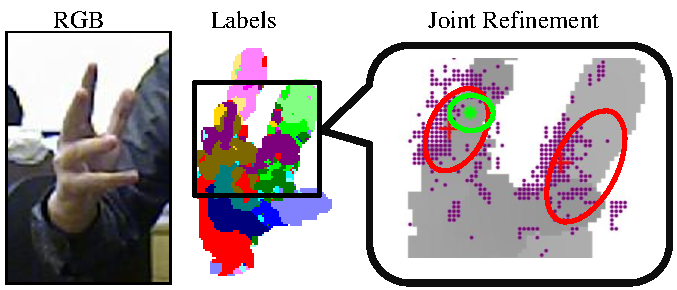
\includegraphics[width=0.8\linewidth]{fig/hand/fig3.pdf}
	\caption{\textbf{Pseudo-kinematic joint refinement algorithm.}}
	\label{fig/hand/refine}
\end{figure}

The true joint usually forms one compact cluster of votes, which leads to a high weighting and low variance in one of the Gaussians. 
On the contrary, a weak detection usually contains scattered votes, indicated by separated means with similar weights. 
A $\testonejoint_{\joint}$ is considered as a high-confidence joint when the Euclidean distance between $\hat{\mu}_{\joint}^{1}$ and $\hat{\mu}_{\joint}^{2}$ is smaller than a predefined threshold $\testqualthres$. The output joint location $\testonejoint_{\joint}$ from the \STR\ forest is computed as
\begin{equation}
	\begin{aligned}
	\testonejoint_{\joint} = &  
	\begin{cases}
		\hat{\mu}_{\joint}^{1} & \mbox{ if } ||\hat{\mu}_{\joint}^{1} - \hat{\mu}_{\joint}^{2}||_2 < \testqualthres \mbox{ and } \hat{\rho}_{\joint}^{1} \ge \hat{\rho}_{\joint}^{2}, \\[3mm] 
		\hat{\mu}_{\joint}^{2} & \mbox{ if } ||\hat{\mu}_{\joint}^{1} - \hat{\mu}_{\joint}^{2}||_2 < \testqualthres \mbox{ and } \hat{\rho}_{\joint}^{1} < \hat{\rho}_{\joint}^{2}, \\[3mm] 
		\mbox{undefined$\;^{\dagger}$} & \mbox{ otherwise }. 
	\end{cases}\\
	& \parbox{0.7\linewidth}{\small $\dagger$: Estimated by kinematic joint refinement algorithm}
	\end{aligned}
	\label{eqn/hand/highconf}
\end{equation}
For a high-confident $j$-th joint, the final output location $\testonejoint_{\joint}$ is represented by the mean of the dominating Gaussian in $\testGMM_{\joint}$. Otherwise, low-confidence joints, \ie undefined joints in equation \ref{eqn/hand/highconf}, are computed using the kinematic joint refinement algorithm in section \ref{sec/hand/kjr}. 

% done 
\subsection{Kinematic joint refinement} 
\label{sec/hand/kjr} 

Whilst locations of high-confidence joints are finalised from the regression forest, the joint refinement process is performed to estimate the remaining low-confidence joints. 
The high-confidence joints are matched to the means $\{\mu_{\testviewlabel}^{1}\dots\mu_{\testviewlabel}^{\ngmm}\}$ in the kinematic model $\GMM_{\testviewlabel}$, where their nearest neighbours are found by least squares fitting, with a direct similarity transformation $\mathbf{T}$.  
Only the high-confident joint locations are used in the above nearest neighbour matching, and the low-confident joint locations are masked out. 
Given the nearest Gaussian $\{\mu_{\testviewlabel}^{nn}, \Sigma_{\testviewlabel}^{nn}\}$ of the high-confidence joints, one of the two Gaussians in section \ref{sec/hand/strtesting} is selected: 
%each remaining low-confidence joint $\testonejoint_{\joint}$ are computed as
\begin{equation}
		\{\tilde{\mu}, \tilde{\Sigma}\} 
		= \argmin_{\{\mu, \Sigma\} \in \{\hat{\mu}_{\joint}^{1}, \hat{\Sigma}_{\joint}^{1}\},  \{\hat{\mu}_{2}\, \hat{\Sigma}_{2}\}}  
		\big|\big|\mathbf{T}\mu - \mu_{\testviewlabel}^{nn}[\joint]\big|\big|^2_2.
		\label{eqn/hand/refine1}
\end{equation}
The distribution $\{\tilde{\mu}, \tilde{\Sigma}\}$ is one of the Gaussian components in $\testGMM_{\joint}$ that is closer to the corresponding $\joint$-th joint location in $\{\mu_{\testviewlabel}^{nn}[\joint] \in \mathbb{R}^{3}, \Sigma_{\testviewlabel}^{nn}[\joint] \in \mathbb{R}^{3\times3}\}$ taken from $\{ \mu_{\testviewlabel}^{nn}, \Sigma_{\testviewlabel}^{nn} \} $. However, when a joint is fully occluded, its detection result in equation \ref{eqn/hand/refine1} become unreliable because the regression forest does not consider complete occlusion.   
As a result, the final output of a low-confidence joint $\testonejoint_{l}$ is recovered by merging the Gaussians in equation \ref{eq:refine2} (\cf equation \ref{eqn/body/combine}): 
\begin{equation}
	\testonejoint_{\joint} =
	\bigg(\tilde{\Sigma}^{-1} + \left(\Sigma_{\testviewlabel}^{nn}[\joint]\right)^{-1}\bigg)^{-1}  \bigg( \tilde{\Sigma} \mu_{\testviewlabel}^{nn}[\joint] + \Sigma_{\testviewlabel}^{nn}[\joint]\tilde{\mu}\bigg).
	\label{eq:refine2}
\end{equation}

Figure \ref{fig/hand/refine} illustrates the process of refining a low-confidence joint. The middle proximal joint is occluded by the index finger as seen in the RGB image; the Gaussians components in $\testGMM_{\joint}$ is represented by the red crosses (mean) and ellipses (variance). The final output is computed by merging the nearest neighbour obtained from $\GMM$, \ie $\{\mu_{\testviewlabel}^{nn}[\joint], \Sigma_{\testviewlabel}^{nn}[\joint]\}$ (the green Gaussian), and the closer Gaussian in $\testGMM_{\joint}$ (the left red Gaussian).  
The procedures of refining output poses $\testjoint$ are stated in algorithm \ref{alg/hand/testing}.  

\begin{algorithm}
	\KwData{Vote vectors obtained from passing down the testing image to the \STR\ forest.}
	\KwResult{The output pose $\testjoint:\mathbb{R}^{3\times16}$.} 
	Extract patches $\testpatchset$ from depth image $\testimg$ \\ 
	\ForEach{$\testpatch \in \testpatchset$}{
		Compute the viewpoint $\testviewlabel$ and joint $\testjointlabel$. \\ 
		Each $\testpatch$ votes at the leaf nodes
	}
	\ForEach{ Set of voting vectors for the $\joint$-th joint}{
		Learn a $2$-part GMM $\testGMM_{\joint}$ of the voting vectors\\ 
		\If{$||\hat{\mu}_{\joint}^{1} - \hat{\mu}_{\joint}^{2}||^2_2 < \testqualthres$}{
			The $\joint$-th joint is a high-confidence joint\\
			Compute the $\joint$-th joint location. (Equation \ref{eqn/hand/highconf}) 
		}\Else{
			The $\joint$-th joint is a low-confidence joint
		}
	}
	Find the nearest neighbour $\{\mu_{\testviewlabel}^{nn},\Sigma_{\testviewlabel}^{nn}\}$ by matching the high-confidence joints with $\GMM_{\testviewlabel}$\\ 
	Update the remaining low-confidence joint (Equation \ref{eqn/hand/refine1} and \ref{eq:refine2}) \\
	\caption{\textbf{Joint detection and pose refinement.}} 
	\label{alg/hand/testing}
\end{algorithm}

\section{Experiments}
\label{sec/hand/experiments}

% done 
\subsection{Evaluation dataset} 

Synthetic training data $\synset$ was rendered using an articulated hand model as shown in figure \ref{fig/hand/label}. 
Instead of adjusting individual joints, each finger was controlled by a bending parameter, such that only realistic articulations, \ie poses that can be performed by a real hand, were recorded in the training dataset. 
In order to handle the shape variations in realistic environments, mild shape randomisation is applied to the articulated hand model, when generating the depth images in dataset $\synset$. 
%Different poses performed by the articulated model were subsequently projected to depth images.
Subsequently, a synthetic dataset $\synset$ was generated by projecting the articulated model, of different poses, to depth images. In this work, $\synset$ contained $\nsynperview$ depth images per viewpoint, the size of $\synset$ was $\nsynperview \times 3 \times 5 \times 9 = 337.5K$.  

\begin{figure}[ht]
	\centering
	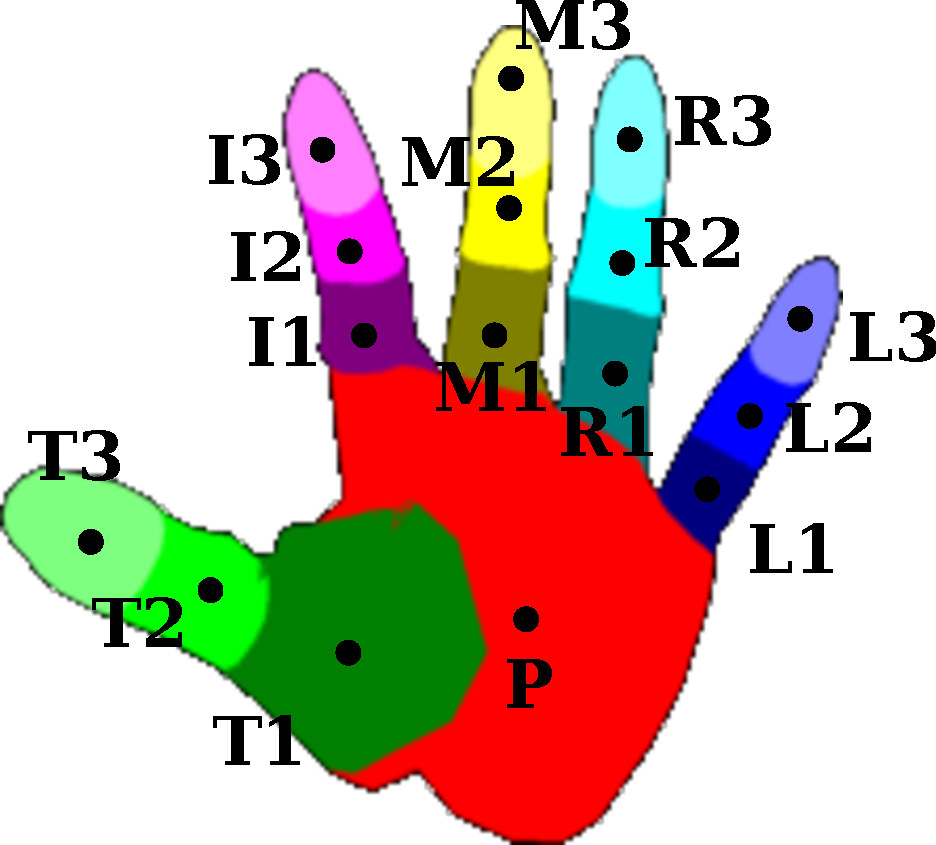
\includegraphics[width=0.32\linewidth]{fig/hand/hand.pdf}
	\caption{\textbf{Colour codes and labels of the 16 hand regions.}}
	\label{fig/hand/label}
\end{figure}

Meanwhile, realistic data $\realset$ was captured using an Asus Xtion depth sensor. 
There were about $600$ frames per viewpoint, thus the size of $\realset$ is $81K$. 
Within $\realset$, about $20\%$ of the frames in $\realset$ are labelled. 
The number of labelled sample $|\reallset|$ is around $10K$.    
Since labels can be reused for the in-plane rotationally symmetric images (same yaw and pitch, but different roll), only around $1.2K$ of data are actually hand-labelled.    

Visible joints in $\reallset$ were annotated manually using 3D coordinates. However, annotation of occluded joints were labelled using the $(x,y)$ coordinates initially.  
Realistic-synthetic associations $\assoc$ and the remaining $z$-coordinates in $\reallset$ were computed simultaneously by matching visible joint locations with $\synset$, using least squares and a direct similarity transform, similar to kinematic joint refinement in section \ref{sec/hand/kjr}. 
Consequently, each data point in $\reallset$ was paired with its closest match $\patch_{syn} \in \synset$, and its occluded $z$ coordinates were approximated by the corresponding $z$ coordinates of $\patch_{syn}$.  
A joint was modelled as a 3D truncated Gaussian distribution centred at the joint location, while its variance was defined empirically according to the structure of human hands. Foreground pixels were clustered into one of these distributions and therefore assigned with labels $\jointlabel$. For example, the palm label usually contributed a larger region than the fingertip labels, due to the large variance in the palm joint.

Three different sequences (sequence $A$,$B$ and $C$) were recorded and labelled needs 50, 1000 and 240 frames respectively.  Sequence $A$ was captured with a static viewpoint for the single-view experiment. Sequence $B$ features various viewpoint variations and sequence $C$ contains abrupt changes in both viewpoint and scale. In the experiments, 3 trees were trained with maximum depth varying from 16 (single-view experiment) to 24 (multi-view experiment), depending on the amount of training data.

% done 
\subsection{Single view experiment} 

\begin{figure}[ht]
	\centering
	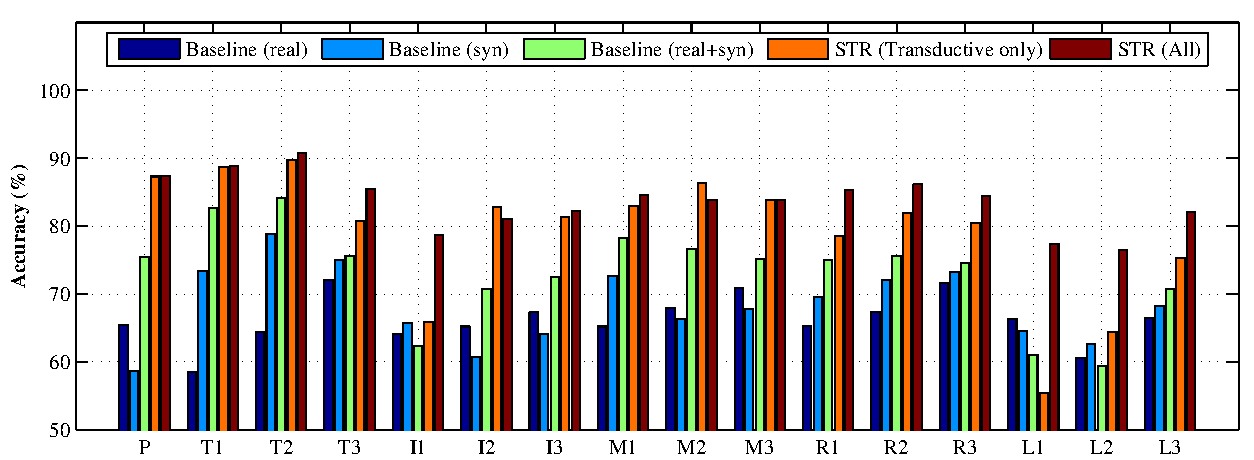
\includegraphics[width=1\linewidth]{fig/hand/singleview.pdf}
	\caption{\textbf{Joint classification accuracy of the single view sequence.}}
	\label{fig/hand/single}
\end{figure}

The proposed approach was evaluated under a single view scenario, comparing with the traditional regression forest algorithm of Gall \etal \cite{Gall2011} as a baseline. Since there was only one viewpoint in testing sequence $A$, $\viewterm$ in equation \ref{eqn/hand/qualityfunction1} did not affect the experimental results. In other words, the proposed method and the baseline algorithm only differed in joint regression and classification, hence only $\classterm$,$\regterm$, $\pairterm$ and $\usterm$ were actually used in this experiment.    

Performances of candidate algorithms were measured by their pixel-wise classification accuracy per joint \cite{Shotton2011}. Figure \ref{fig/hand/single} shows the classification accuracy plots of the algorithm evaluated in this experiment.  
It demonstrates the strengths of realistic-synthetic fusion and semi-supervised learning. 
Accuracy of baseline method was improved by simply including both domains in training without any algorithmic changes. 

The transductive learning term $\pairterm$ improved the accuracy substantially, particularly for the finger tips which are less robust in the baseline algorithms.  
By coupling realistic data with synthetic data, the transductive term $\pairterm$ effectively learns the discrepancies between the domains.
%, which is important in recognising noisy and strongly occluded fingers.
From figure \ref{fig/hand/single}, some joints are often mislabelled as other more dominating joints after transductive learning, \eg joints in little finger tip (L3) and index proximal (I1). 
Nevertheless, semi-supervised learning significantly corrects those joints after transductive learning. To summarise, semi-supervised learning complements transductive learning by modelling the intermediate poses between the sparsely labelled realistic data.    

%\paragraph{Experiment on Data-driven Joint Refinement}
%A fully-labelled, multiview video sequence is recorded to evaluate the overall performances of the approaches.  

\subsection{Multiple view experiment}  

In the multi-view experiment, the proposed approach was compared with the state-of-the-art by Oikonomidis \etal (FORTH algorithm, a tracking-based generative model) \cite{Oikonomidis2011} under two challenging multi-view scenarios. Quantitative and qualitative evaluations were performed to provide a comprehensive comparison of the methods. 

Hand articulations were estimated from the multi-view testing sequences, \ie sequence $B$ and $C$, by both of the methods. 
Sequence $B$ contains long and continuous pose and viewpoint changes, while abrupt viewpoint changes and strong occlusions are observed in sequence $C$.  
Since FORTH requires manual initialisation, the testing sequences are designed such that they start with a fixed initialisation pose and position, in order to facilitate a fair comparison.   
In this experiment, pose estimation accuracy was measured by joint localisation error \cite{Oikonomidis2011}.

\subsubsection{Quantitative results}

Figure \ref{fig/hand/multiquantb} and \ref{fig/hand/multiquantc} show the average localisation errors of testing sequence $B$ and $C$ respectively. It also shows the same error graphs from a stable joint (palm, $P$) and a difficult joint (index finger tip, $I3$). The proposed \STR\ forest, together with the data-driven kinematic joint refinement, outperform FORTH in all aspects, especially for the finger tip joints that are noisy and frequently occluded. Since the proposed approach is frame-based, even though a few large estimation errors are observed, they can be recovered quickly without drifting.    

Experiments with sequence $C$ justify the advantages of the proposed system over tracking-based methods. In the first $200$ frames, \STR\ forest with joint refinement perform just slightly better than FORTH. However, localisation errors in FORTH accumulate after an abrupt change in the testing sequence, and the incorrect pose does not recover.
% the errors have not been recovered since then. 
Since tracking-based approaches rely on previous results to optimise the current hypothesis iteratively, estimation errors amass and drifting issue worsens over time. On the contrary, frame-based discriminative approaches consider each frame as an independent input, enabling fast error recovery at the expense of a smooth and continuous output, hence small jitters are observed from the hand pose estimation results.  

In this experiment, the proposed joint refinement scheme improves the joint estimation accuracy in general, as illustrated in figure \ref{fig/hand/multiquantb} and \ref{fig/hand/multiquantc}. 
Some large classification errors, \eg figure \ref{fig/hand/multiquantb2}, are corrected after applying joint refinement. It implies that the joint refinement process not only improves the accuracy of joint, but also prevents incorrect detections by validating the output of \STR\ forest with kinematic constraints.

\begin{figure}[ht]
	\centering
	\subcaptionbox{Test sequence $B$ (Average error)\label{fig/hand/multiquantb1}}{
		\centering
		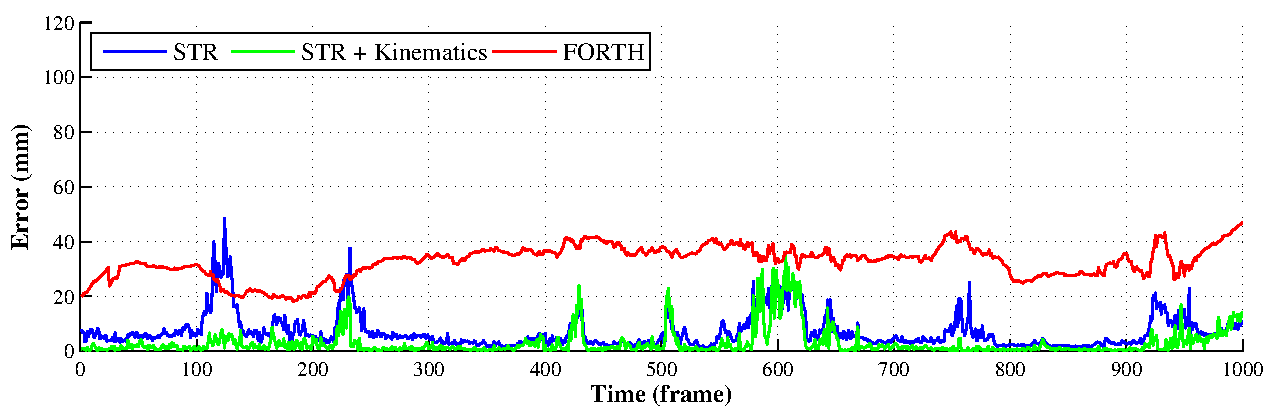
\includegraphics[width=0.95\linewidth]{fig/hand/sq1_avg.pdf}
	}
	\subcaptionbox{Test sequence $B$ (Palm)\label{fig/hand/multiquantb2}}{
		\centering
		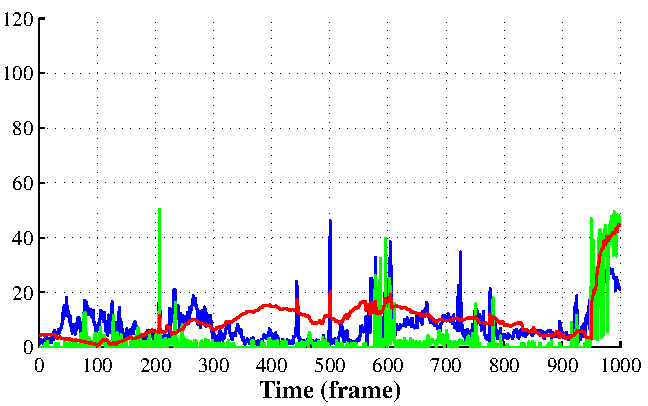
\includegraphics[width=0.95\linewidth]{fig/hand/sq1_palm.pdf}
	}
	\subcaptionbox{Test sequence $B$ (Index finger tip)\label{fig/hand/multiquantb3}}{
		\centering
		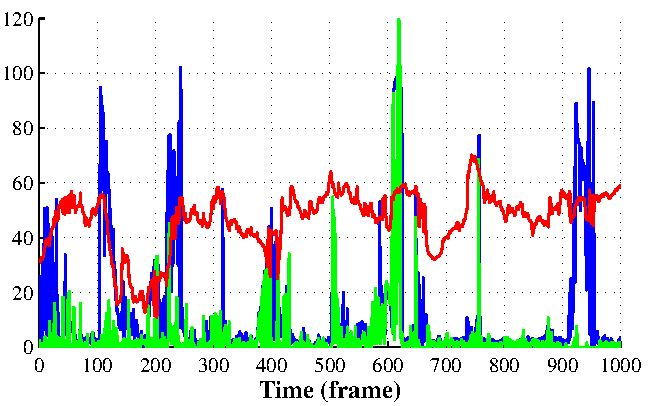
\includegraphics[width=0.95\linewidth]{fig/hand/sq1_tip.pdf}
	}
	\caption{\textbf{Quantitative hand pose estimation results --- Sequence $B$}}
	\label{fig/hand/multiquantb}
\end{figure}

\begin{figure}[ht]
	\centering
	\subcaptionbox{Test sequence $C$ (Average error)\label{fig/hand/multiquantc1}}{
		\centering
		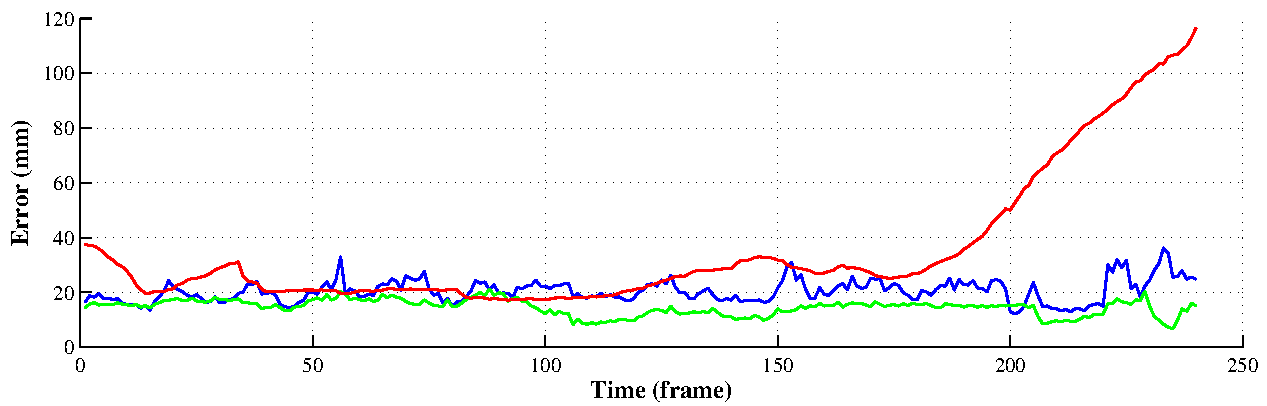
\includegraphics[width=0.95\linewidth]{fig/hand/sq2_avg.pdf}
	}
	\subcaptionbox{Test sequence $C$ (Palm)\label{fig/hand/multiquantc2}}{
		\centering
		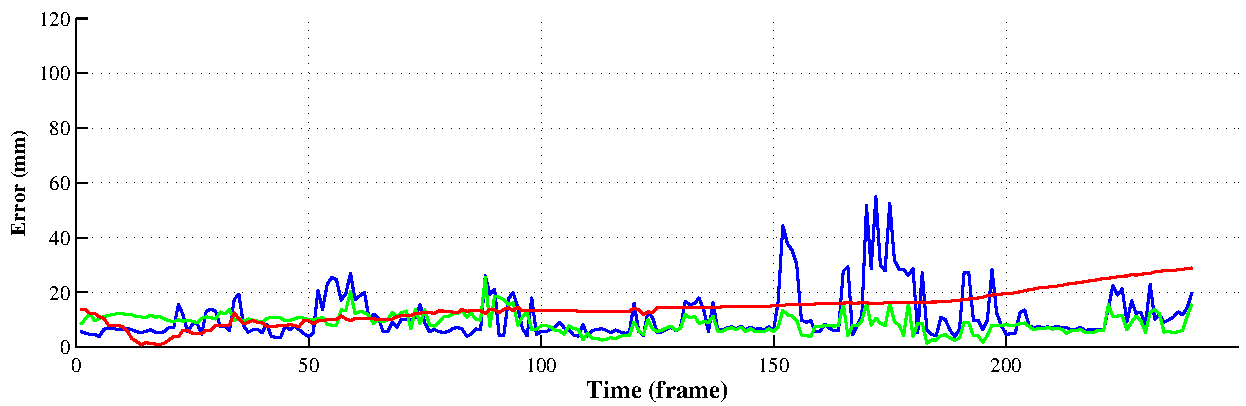
\includegraphics[width=0.95\linewidth]{fig/hand/sq2_palm.pdf}
	}
	\subcaptionbox{Test sequence $C$ (Index finger tip)\label{fig/hand/multiquantc3}}{
		\centering
		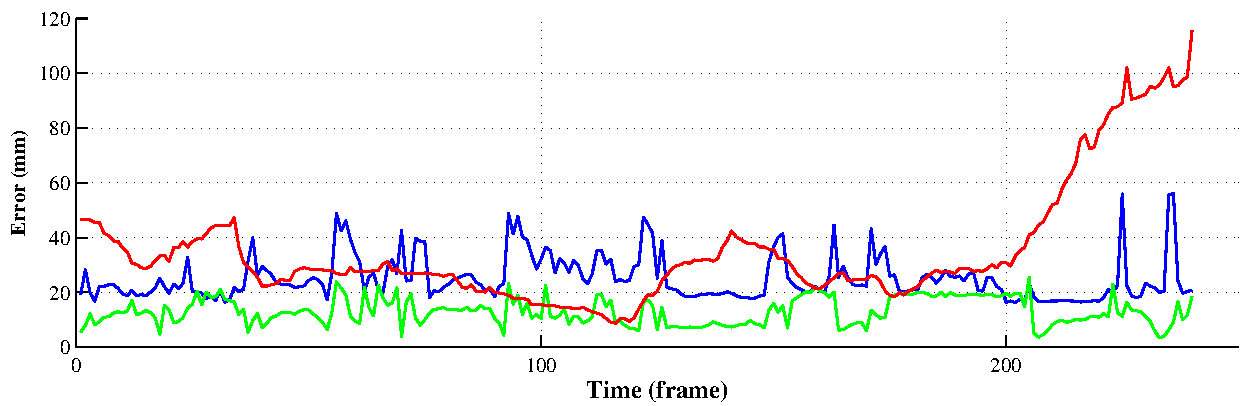
\includegraphics[width=0.95\linewidth]{fig/hand/sq2_tip.pdf}
	}
	\caption{\textbf{Quantitative hand pose estimation results --- Sequence $C$.}}
	\label{fig/hand/multiquantc}
\end{figure}


\subsubsection{Qualitative analysis} 

The proposed pose estimation system was also evaluated qualitatively, figure \ref{fig/hand/multiqual} displays some of the experimental results extracted from testing sequence $B$ and $C$.
In figure \ref{fig/hand/multiqual}, hands are cropped from the original images for better visualisation ($135\times135$ pixels for sequence $B$, $165\times165$ pixels for sequence $C$). During the experiment, the size of the original images (RGB and depth) is $640\times480$ pixels.
Figure \ref{fig/hand/multiqual}(a) and (b) show the pose estimation results of the same articulation from different view points.  
Figure \ref{fig/hand/multiqual}(d) shows a frame at the beginning of test sequence $B$, both approaches obtain accurate hand articulations initially. However, the performance of FORTH declined rapidly in the middle of the sequence when its tracking algorithm lost target and failed to recognise a correct pose in figure \ref{fig/hand/multiqual}(e), yet the \STR\ forest approach still gives correct results. In addition, strong occlusions are shown in figure \ref{fig/hand/multiqual}(f), where FORTH did not work well but the \STR\ forest gave the correct pose. In figure \ref{fig/hand/multiqual}, however, both approaches did not produce very accurate results due to strong motion blur, which is indicated by a large blank region in the corresponding depth image.   

With respect to run-time performance, the proposed \STR\ forest estimated one hand pose at about $25$FPS on an Intel I7 PC without GPU acceleration, whilst the FORTH algorithm ran at $6$FPS on the same hardware configuration plus GPU acceleration (NVidia GT 640). 

%\begin{figure}[ht]
%	\centering
%	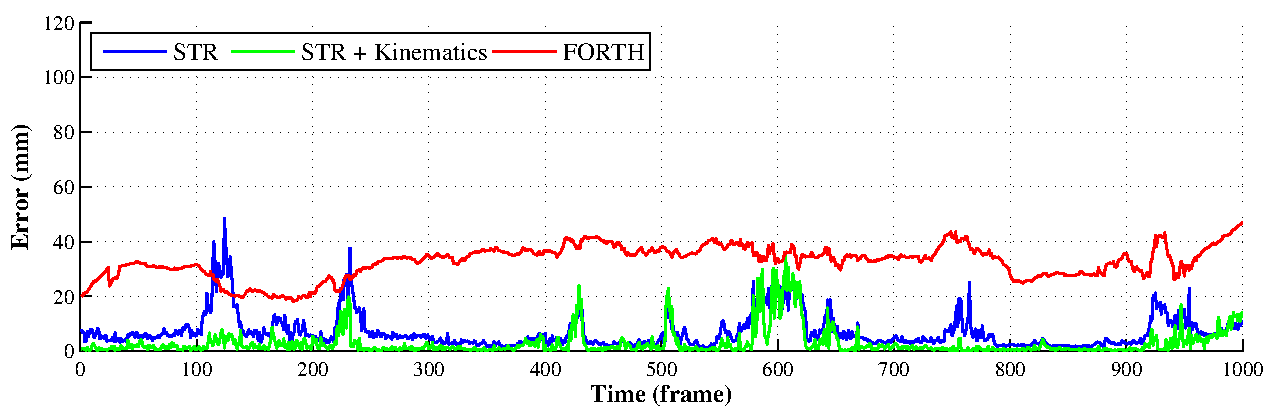
\includegraphics[width=0.33\linewidth]{fig/hand/sq1_avg.pdf}  
%	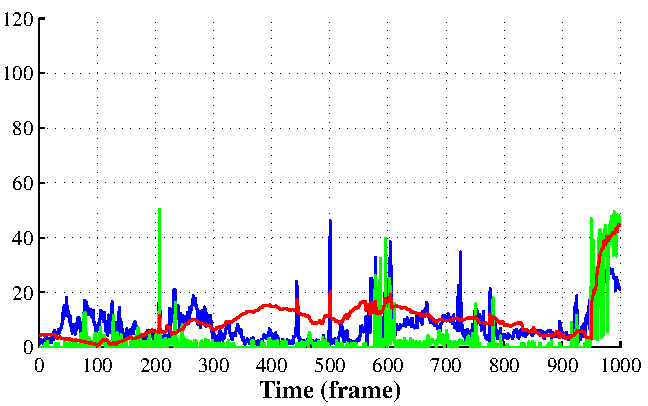
\includegraphics[width=0.31\linewidth]{fig/hand/sq1_palm.pdf} 
%	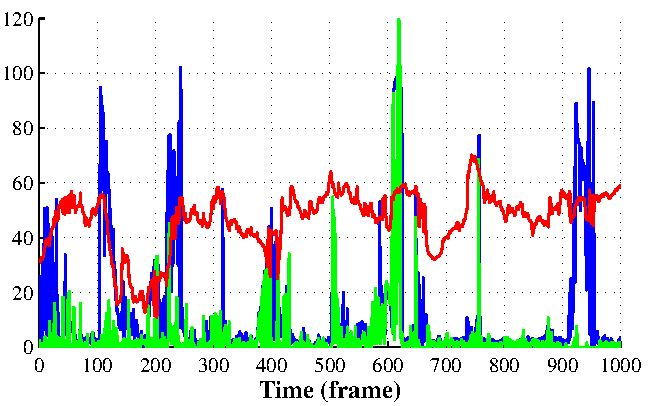
\includegraphics[width=0.31\linewidth]{fig/hand/sq1_tip.pdf} \\
%	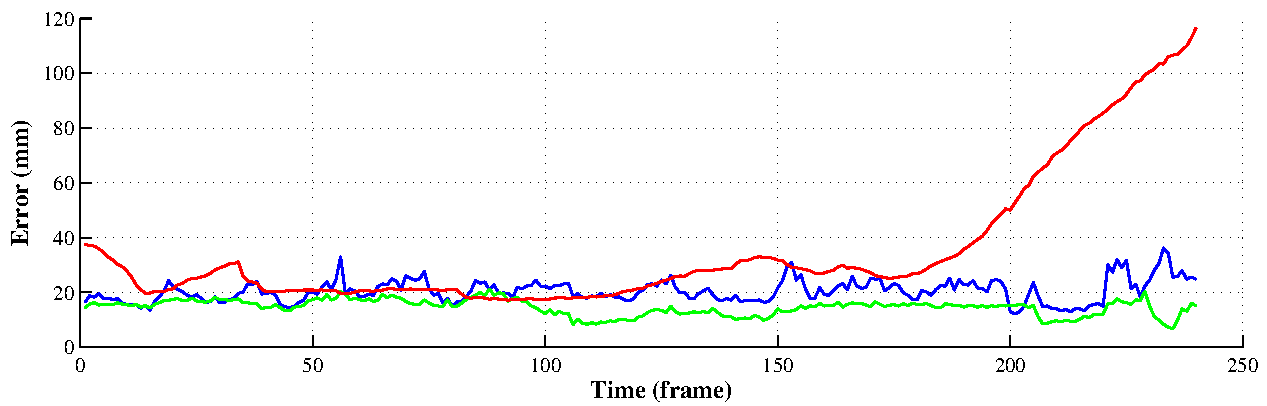
\includegraphics[width=0.33\linewidth]{fig/hand/sq2_avg.pdf} 
%	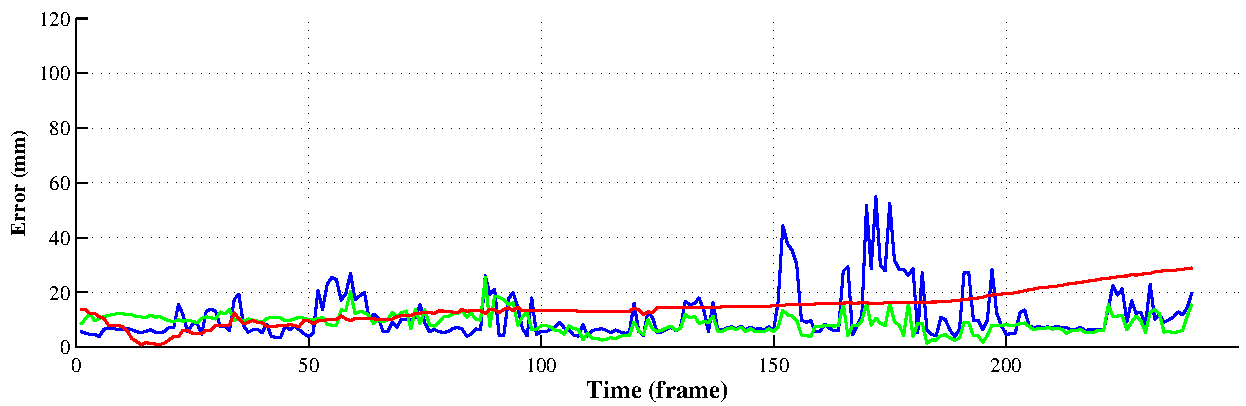
\includegraphics[width=0.31\linewidth]{fig/hand/sq2_palm.pdf}
%	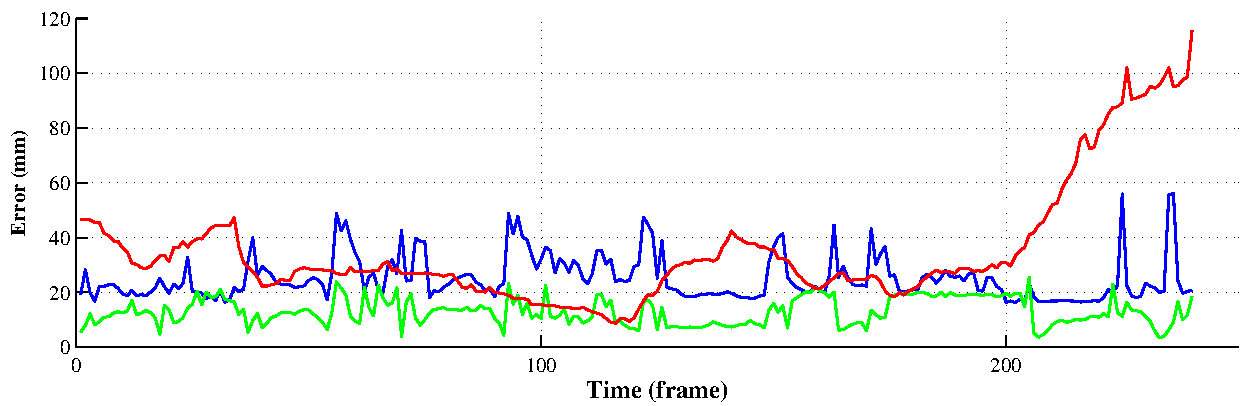
\includegraphics[width=0.31\linewidth]{fig/hand/sq2_tip.pdf} 
%	\caption{Joint localisation errors of the multiview testing squences.}
%	\label{fig/hand/multiquant}
%\end{figure}

% 3 x 4 or 4 x 4 image array (RGB, Depth, Ours, FORTH), I expect half a page  
% show two similar poses with similar viewpoints 
% show a pose with heavy occlusion 
% shows FORTH gives large error when it loses track 
\begin{figure}
	\centering
	\begin{tabular}{@{}cc@{}c@{}c@{}c@{}c@{}}
		\textbf{Frame} & \textbf{RGB} & \textbf{Depth} & \textbf{FORTH} & \textbf{Classification} & \textbf{3D Pose} \\ 
		\hline 
		\multicolumn{6}{c}{\textbf{Testing hand sequence $B$}} \\ 
		\hline 
		\raisebox{1.3cm}{\parbox{2cm}{\centering (a)\\Frame 303}} & 
		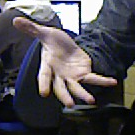
\includegraphics[width=2.35cm]{fig/hand/qual/rgb/image_0303.png} &
		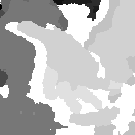
\includegraphics[width=2.35cm]{fig/hand/qual/depth/image_0303.png} &
		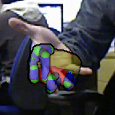
\includegraphics[width=2.35cm]{fig/hand/qual/forth/image_0303.png} &
		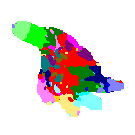
\includegraphics[width=2.35cm]{fig/hand/qual/class/class-303.png} &
		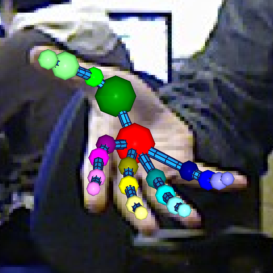
\includegraphics[width=2.35cm]{fig/hand/qual/vote/image_0303.png}
		\phantomsubcaption\label{fig/hand/multi1} \\
		\raisebox{1cm}{\parbox{2cm}{\centering (b)\\Frame 520}} & 
		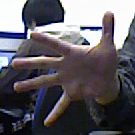
\includegraphics[width=2.35cm]{fig/hand/qual/rgb/image_0520.png} &
		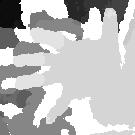
\includegraphics[width=2.35cm]{fig/hand/qual/depth/image_0520.png} &
		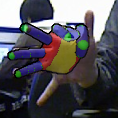
\includegraphics[width=2.35cm]{fig/hand/qual/forth/image_0520.png} &
		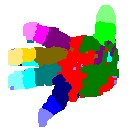
\includegraphics[width=2.35cm]{fig/hand/qual/class/class-520.png} &
		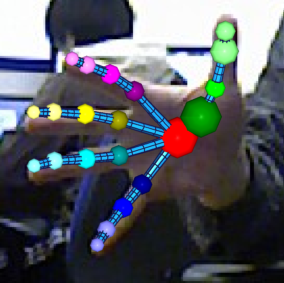
\includegraphics[width=2.35cm]{fig/hand/qual/vote/image_0520.png}
		\phantomsubcaption\label{fig/hand/multi2} \\
		\raisebox{1cm}{\parbox{2cm}{\centering (c)\\Frame 825}} & 
		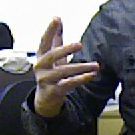
\includegraphics[width=2.35cm]{fig/hand/qual/rgb/image_0825.png} &
		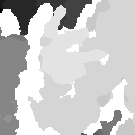
\includegraphics[width=2.35cm]{fig/hand/qual/depth/image_0825.png} &
		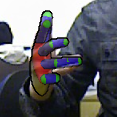
\includegraphics[width=2.35cm]{fig/hand/qual/forth/image_0825.png} &
		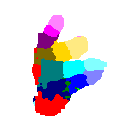
\includegraphics[width=2.35cm]{fig/hand/qual/class/class-825.png} &
		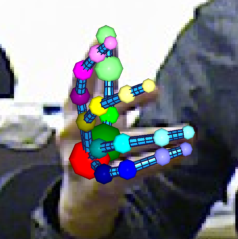
\includegraphics[width=2.35cm]{fig/hand/qual/vote/image_0825.png}
		\phantomsubcaption\label{fig/hand/multi3} \\
		\raisebox{1cm}{\parbox{2cm}{\centering (d)\\Frame 946}} & 
		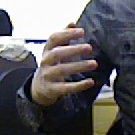
\includegraphics[width=2.35cm]{fig/hand/qual/rgb/image_0946.png} &
		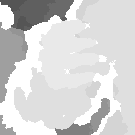
\includegraphics[width=2.35cm]{fig/hand/qual/depth/image_0946.png} &
		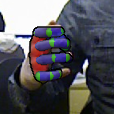
\includegraphics[width=2.35cm]{fig/hand/qual/forth/image_0946.png} &
		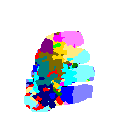
\includegraphics[width=2.35cm]{fig/hand/qual/class/class-946.png} &
		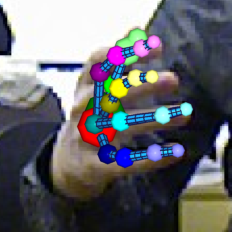
\includegraphics[width=2.35cm]{fig/hand/qual/vote/image_0946.png}
		\phantomsubcaption\label{fig/hand/multi4} \\
		\raisebox{1cm}{\parbox{2cm}{\centering (e)\\Frame 996}} & 
		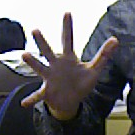
\includegraphics[width=2.35cm]{fig/hand/qual/rgb/image_0996.png} &
		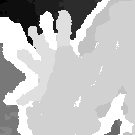
\includegraphics[width=2.35cm]{fig/hand/qual/depth/image_0996.png} &
		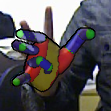
\includegraphics[width=2.35cm]{fig/hand/qual/forth/image_0996.png} &
		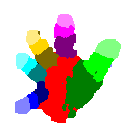
\includegraphics[width=2.35cm]{fig/hand/qual/class/class-996.png} &
		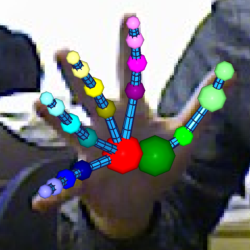
\includegraphics[width=2.35cm]{fig/hand/qual/vote/image_0996.png}
		\phantomsubcaption\label{fig/hand/multi5} \\ 
		\hline 
		\multicolumn{6}{c}{\textbf{Testing hand sequence $C$}} \\ 
		\hline 
		\raisebox{1cm}{\parbox{2cm}{\centering (f)\\Frame 198}} &
		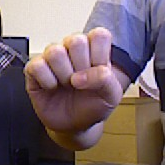
\includegraphics[width=2.35cm]{fig/hand/qual/rgb/image_0198.png} &
		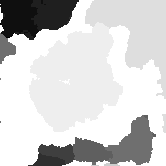
\includegraphics[width=2.35cm]{fig/hand/qual/depth/image_0198.png} &
		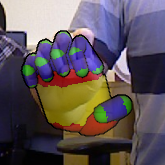
\includegraphics[width=2.35cm]{fig/hand/qual/forth/image_0198.png} &
		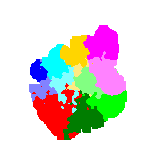
\includegraphics[width=2.35cm]{fig/hand/qual/class/class-198.png} &
		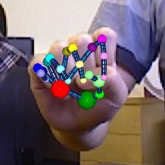
\includegraphics[width=2.35cm]{fig/hand/qual/vote/image_0198.png} 
		\phantomsubcaption\label{fig/hand/multi6} \\
		\raisebox{1cm}{\parbox{2cm}{\centering (g)\\Frame 440}} & 
		\includegraphics[width=2.35cm]{fig/hand/qual/rgb/image_0440.png} &
		\includegraphics[width=2.35cm]{fig/hand/qual/depth/image_0440.png} &
		\includegraphics[width=2.35cm]{fig/hand/qual/forth/image_0440.png} &
		\includegraphics[width=2.35cm]{fig/hand/qual/class/class-440.png} &
		\includegraphics[width=2.35cm]{fig/hand/qual/vote/image_0440.png} 
		\phantomsubcaption\label{fig/hand/multi7} \\
	\end{tabular}
	\caption{\textbf{Qualitative experimental results of the multi-view experiment.} For each row, from left to right: RGB image, depth image, hand pose from FORTH, joint labels from the proposed method, final hand pose output of the proposed method.}
	\label{fig/hand/multiqual}
\end{figure} 
 

% done 
\section{Summary}

The chapter investigates the problem of pose estimation of human hand pose from depth image sequences. 
Despite sharing many similarities with body pose estimation, practical 3D hand pose estimation is still far from mature, primarily due to the characteristics of hand poses, in which occlusion and noise prevail. 
Furthermore, the discrepancies between realistic and synthetic data also undermine the performances of existing systems. 

Dealing with the above issues, this work introduces a semi-supervised transductive approach for articulated hand pose estimation. A novel discriminative pose estimator, namely \STR\ forest, is proposed to infer hand poses using both realistic and synthetic training data. 
With transductive learning, the \STR\ forest recognises a wide range of poses from a small labelled realistic dataset by linking its data points to a large synthetic dataset.
Semi-supervised learning is also applied to fully utilise the sparsely labelled realistic dataset. 
To improve the estimation accuracy of heavily occluded hand poses, a data-driven pseudo-kinematic technique is used to correct the occluded joints.  

The proposed hand pose estimation system was evaluated with respect to different challenging environments. From the quantitative and qualitative analyses, it demonstrated promising results in estimating articulated hand poses from noisy and strongly occluded data.  
It also achieved superior accuracy and run-time performance compared with current state-of-the-art approaches.  
